\documentclass[12pt, hidelinks]{article}
\usepackage[brazil]{babel}
\usepackage[utf8]{inputenc}
\usepackage{amsmath}
\usepackage{natbib}
\usepackage{listings}
\usepackage{color}

\definecolor{codegreen}{rgb}{0,0.6,0}
\definecolor{codegray}{rgb}{0.5,0.5,0.5}
\definecolor{codepurple}{rgb}{0.58,0,0.82}
\definecolor{backcolour}{rgb}{0.95,0.95,0.92}

\lstdefinestyle{mystyle}{
  backgroundcolor=\color{backcolour},
  commentstyle=\color{codegreen},
  keywordstyle=\color{red},
  numberstyle=\tiny\color{codegray},
  stringstyle=\color{codepurple},
  basicstyle=\footnotesize,
  breakatwhitespace=false,
  breaklines=true,
  captionpos=b,
  keepspaces=true,
  numbers=left,
  numbersep=5pt,
  showspaces=false,
  showstringspaces=false,
  showtabs=false,
  tabsize=2,
  extendedchars=true,
  literate={á}{{\'a}}1 {ã}{{\~a}}1 {õ}{{\~o}}1 {é}{{\'e}}1 {ç}{{\c{c}}}1,
}

\lstset{style=mystyle}
\usepackage{url}
\usepackage{amsmath}
\usepackage{float}
\usepackage{graphicx}
\graphicspath{{images/}}
\usepackage{parskip}
\usepackage{fancyhdr}
\usepackage{vmargin}
\usepackage{hyperref}
\setmarginsrb{3 cm}{2.5 cm}{3 cm}{2.5 cm}{1 cm}{1.5 cm}{1 cm}{1.5 cm}


\title{Interpolação Polinomial}         % Title
\author{Wilton Rodrigues}								% Author
\date{\today}											      % Date

\makeatletter
\let\thetitle\@title
\let\theauthor\@author
\let\thedate\@date
\makeatother

\pagestyle{fancy}
\fancyhf{}
\lhead{\centering{\thetitle}}
\cfoot{\thepage}

\begin{document}

%%%%%%%%%%%%%%%%%%%%%%%%%%%%%%%%%%%%%%%%%%%%%%%%%%%%%%%%%%%%%%%%%%%%%%%%%%%%%%%%%%%%%%%%%

\begin{titlepage}
  \centering
  \begin{figure}[H]
    \centering
    
\includegraphics[width=0.7\textwidth]{figuras/logo.png}\\[2.0 cm]
  \end{figure}
  \textsc{\LARGE Universidade de Brasília}\\[2.5 cm]	% University Name
  \textsc{\Large Relatório de atividade do módulo 4}\\[0.5 cm]				% Activity name
  \textsc{\large Métodos Numéricos para Engenharia}\\[1.5 cm]				% Course Name
  \rule{\linewidth}{0.2 mm} \\[0.4 cm]
  {\huge \bfseries \thetitle}\\
  \rule{\linewidth}{0.2 mm} \\[2.5 cm]

  \begin{minipage}{0.4\textwidth}
    \begin{flushleft} \large
      \emph{Aluno:}\\
      \theauthor
    \end{flushleft}
  \end{minipage}
  \begin{minipage}{0.4\textwidth}
    \begin{flushright} \large
      \emph{Matrícula:} \\
      13/0049212									% Your Student Number
    \end{flushright}
  \end{minipage}\\
  \vspace*{0.5in}
  {\large \thedate}\\[0.5 cm]

  \vfill

\end{titlepage}

%%%%%%%%%%%%%%%%%%%%%%%%%%%%%%%%%%%%%%%%%%%%%%%%%%%%%%%%%%%%%%%%%%%%%%%%%%%%%%%%%%%%%%%%%

\section{Introdução}

O objetivo deste relatório é exercitar os conceitos aprendidos em aula, com relação ao tópico: \thetitle.

Interpolar uma função $f(x)$ consiste em aproximar essa função por uma outra função $g(x)$. A função $g(x)$
é então usada em substituição à função $f(x)$.
A necessidade de se efetuar esta substituição surge em várias situações, como por exemplo, quando são
conhecidos somente os valores numéricos da função para um conjunto de pontos e é necessário calcular o
valor da função em um ponto não tabelado.

O problema a ser solucionado é o que trata da seguinte tabela de resultados para a densidade da água, $\rho$, em várias temperaturas, como é mostrado a seguir:
\begin{table}[h]
  \centering
  \begin{tabular}{|c|c|c|c|c|c|c|c|c|c|}
    \hline
      $T$ & 0 & 5 & 10 & 15 & 20 & 25 & 30 & 35 & 40\\
    \hline
      $\rho$ & 0.9999 & 0.9998 & 0.9997 & 0.9991 & 0.9982 & 0.9971 & 0.9957 & 0.9941 & 0.9902\\
    \hline
  \end{tabular}
  \caption{Valores tabelados}
\end{table}

O objetivos deste relatório será, através de interpolação polinomial de 2\textsuperscript{\b{o}} e 3\textsuperscript{\b{o}} graus, obter os valores de $\rho(13)$ e $\rho(27)$. E por fim, apresentar um gráfico com os pontos e os polinômios interpoladores obtidos.

\section{Metodologia}

Baseando-se no método da Interpolação de Lagrange:
\begin{eqnarray}\label{eq:lagrange}
  P(x) = \sum\limits_{i=0}^{n}y_i \frac{L_i(x)}{L_i(x_i)}
\end{eqnarray}
Onde: $L_i(x) = (x - x_0) ... (x - x_i-1)(x - x_i+1) ... (x - x_n)$.

Para $n$ pontos, obtemos um polinômio de grau $n-1$. Baseado nisso, a fim de encontrar o valor de $\rho(13)$, como um polinômio de 2\textsuperscript{\b{o}} utilizaremos os 3 seguintes pontos:

\begin{table}[h]
  \centering
  \begin{tabular}{|c|c|c|c|}
    \hline
      $T$ & 5 & 10 & 15\\
    \hline
      $\rho$ & 0.9998 & 0.9997 & 0.9991\\
    \hline
  \end{tabular}
  \caption{Valores para $\rho(13)$}
\end{table}

Aonde, ao aplicarmos a equação~\eqref{eq:lagrange} obtemos o seguinte resultado:
\begin{eqnarray}\label{eq:pn}
  P(x) = f(x_0)\cdot L_0(x) + f(x_1)\cdot L_1(x) + f(x_2)\cdot L_2(x)
\end{eqnarray}

Onde: \\
$L_0(x) = \frac{(x - x_1)\cdot(x - x_2)}{(x_0 - x_1)\cdot(x_0 - x_2)} = \frac{(x - 10)\cdot(x - 15)}{(5 - 10)\cdot(5 - 15)} = \frac{x^2 - 25x + 150}{50}$\\
$L_1(x) = \frac{(x - x_0)\cdot(x - x_2)}{(x_1 - x_0)\cdot(x_1 - x_2)} = \frac{(x - 5)\cdot(x - 15)}{(10 - 5)\cdot(10 - 15)} = \frac{x^2 - 20x + 75}{-25}$\\
$L_2(x) = \frac{(x - x_0)\cdot(x - x_1)}{(x_2 - x_0)\cdot(x_2 - x_1)} = \frac{(x - 5)\cdot(x - 10)}{(15 - 5)\cdot(15 - 10)} = \frac{x^2 - 15x + 50}{50}$

Obtendo assim o primeiro polinômio interpolador:
\begin{eqnarray}\label{eq:pi1}
  P(x) = 0.9998 \cdot \left(\frac{x^2 - 25x + 150}{50}\right) + 0.9997 \cdot \left(\frac{x^2 - 20x + 75}{-25}\right) + 0.9991 \cdot \left(\frac{x^2 - 15x + 50}{50}\right)
\end{eqnarray}

E para o $\rho(27)$ como um polinômio de 3\textsuperscript{\b{o}} utilizaremos estes 4 pontos:

\begin{table}[h]
  \centering
  \begin{tabular}{|c|c|c|c|c|}
    \hline
      $T$ & 15 & 20 & 25 & 30\\
    \hline
      $\rho$ & 0.9991 & 0.9982 & 0.9971 & 0.9957\\
    \hline
  \end{tabular}
  \caption{Valores para $\rho(27)$}
\end{table}

Aplicando a equação~\eqref{eq:lagrange} mais uma vez:
\begin{eqnarray}\label{eq:pn}
  P(x) = f(x_0)\cdot L_0(x) + f(x_1)\cdot L_1(x) + f(x_2)\cdot L_2(x) + f(x_3)\cdot L_3(x)
\end{eqnarray}

Onde: \\
$L_0(x) = \frac{(x - x_1)\cdot(x - x_2)\cdot(x - x_3)}{(x_0 - x_1)\cdot(x_0 - x_2)\cdot(x_0 - x_3)} = \frac{(x - 20)\cdot(x - 25)\cdot(x - 30)}{(15 - 20)\cdot(15 - 25)\cdot(15 - 30)} = \frac{x^3 - 75x^2 + 1850x - 15000}{-750}$\\
$L_1(x) = \frac{(x - x_0)\cdot(x - x_2)\cdot(x - x_3)}{(x_1 - x_0)\cdot(x_1 - x_2)\cdot(x_1 - x_3)} = \frac{(x - 15)\cdot(x - 25)\cdot(x - 30)}{(20 - 15)\cdot(20 - 25)\cdot(20 - 30)} = \frac{x^3 - 70x^2 + 1575x - 11250}{250}$\\
$L_2(x) = \frac{(x - x_0)\cdot(x - x_1)\cdot(x - x_3)}{(x_2 - x_0)\cdot(x_2 - x_1)\cdot(x_2 - x_3)} = \frac{(x - 15)\cdot(x - 20)\cdot(x - 30)}{(25 - 15)\cdot(25 - 20)\cdot(25 - 30)} = \frac{x^3 - 65x^2 + 1350x - 9000}{-250}$\\
$L_3(x) = \frac{(x - x_0)\cdot(x - x_1)\cdot(x - x_2)}{(x_3 - x_0)\cdot(x_3 - x_1)\cdot(x_3 - x_2)} = \frac{(x - 15)\cdot(x - 20)\cdot(x - 25)}{(30 - 15)\cdot(30 - 20)\cdot(30 - 25)} = \frac{x^3 - 60x^2 + 1175x - 7500}{750}$

Obtendo assim o segundo polinômio interpolador:
\begin{eqnarray}\label{eq:pi2}
  P(x) = 0.9991 \cdot \left(\frac{x^3 - 75x^2 + 1850x - 15000}{-750}\right) + 0.9982 \cdot \left(\frac{x^3 - 70x^2 + 1575x - 11250}{250}\right) + \nonumber \\
  + 0.9971 \cdot \left(\frac{x^3 - 65x^2 + 1350x - 9000}{-250}\right) + 0.9957 \cdot \left(\frac{x^3 - 60x^2 + 1175x - 7500}{750}\right)
\end{eqnarray}

\newpage
\section{Diagrama esquemático de execução}

Nesta seção, encontra-se o fluxo de execução do sistema proposto na equação~\eqref{eq:sistema} utilizando
a linguagem C. Que é apresentada na próxima sessão.

\begin{figure}[!h]
  \centering
  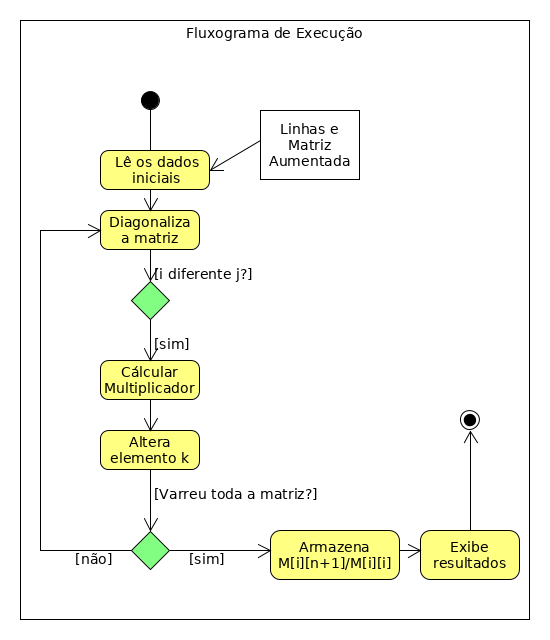
\includegraphics[width=10cm]{figuras/fluxograma.png}\\
  \caption{Fluxo de execução da solução}\label{fig:fluxo}
\end{figure}

A solução elaborada neste relatório funciona da seguinte maneira. É necessário inserir a quantiade de linhas
do sistema de equações lineares, em formato de matriz aumentada, que se quer resolver. Após isso o programa
solicitará a inserção dos elementos de cada uma das linhas da matriz. Após completar a matriz de entrada o
sistema irá fazer a diagonalização de acordo com o método de eliminação de Gaus-Jordan. Onde caso os índices
i e j sejam diferentes, ou seja não fazem parte da diagonal principal, será aplicado o algoritmo de eliminação.
Após haver apenas os elementos da diagonal principal, o método de solução se torna direto e com isso é possível
encontrar os valores da incógnitas que se busca. As limitações do programa são entradas de matrizes de no máximo
10x10 e apenas para equações lineares.

\newpage
\section{Código Fonte}

\lstinputlisting[language=C]{../solution/m4.c}

\newpage
\section{Resultados e discussões}

Nesta seção discutiremos os resultados obtidos após a execução.

\begin{figure}[!h]
  \centering
  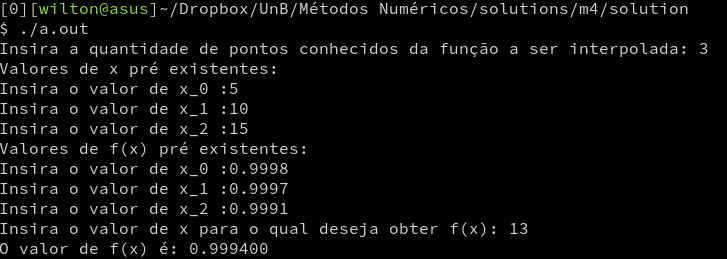
\includegraphics[width=15cm]{figuras/p13.png}\\
  \caption{Resultado da execução do programa}\label{fig:printx}
\end{figure}
Após a execução do programa obtemos os valores dos coeficientes que resulta no seguinte polinômio:
\begin{eqnarray}\label{eq:polinomio}
  C(x) = 0,6523 - 0,2438x + 0,5682x^2
\end{eqnarray}
O resultado encontrado a partir da solução proposta é condizente. Pois ao fazermos a comparação dos valores iniciais com os obtidos através da equação~\eqref{eq:polinomio} encontramos valores bem próximos uns dos outros, como pode ser visto na tabela abaixo:

\begin{table}[h]
  \centering
  \vspace{0.5cm}
  \begin{tabular}{|r|r|r|r|r|r|r|r|r|r|r|}
    \hline
    \multicolumn{11}{|c|}{Valores iniciais do experimento} \\
    \hline
      $\frac{A}{A_1}$ & 0.10 & 0.20 & 0.30 & 0.40 & 0.50 & 0.60 & 0.70 & 0.80 & 0.90 & 1.00\\
    \hline
      $C$ & 0.62 & 0.63 & 0.64 & 0.66 & 0.68 & 0.71 & 0.76 & 0.81 & 0.89 & 1.00\\
    \hline
    \multicolumn{11}{|c|}{Valores obtidos após o método} \\
    \hline
      $\frac{A}{A_1}$ & 0.10 & 0.20 & 0.30 & 0.40 & 0.50 & 0.60 & 0.70 & 0.80 & 0.90 & 1.00\\
    \hline
      $C$ & 0.63 & 0.63 & 0.63 & 0.65 & 0.67 & 0.71 & 0.76 & 0.82 & 0.89 & 0.98\\
    \hline
  \end{tabular}
  \caption{Valores experimentais e de regressão}
\end{table}

\newpage
E também graficamente, como é mostrado abaixo:
\begin{figure}[!h]
  \centering
  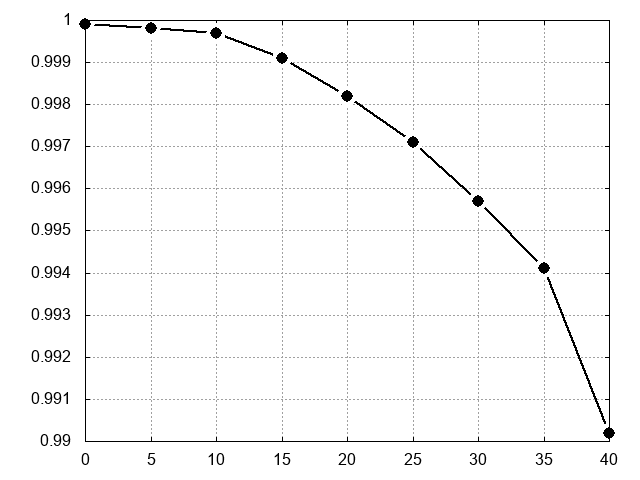
\includegraphics[width=12cm]{figuras/graph.png}\\
\end{figure}

Sendo assim, o objetivo proposto no início do relatório foi satisfatoriamente alcançado.

\newpage
\section{Ferramentas}
Todas as ferramentas utilizadas neste relatório são ferramentas open source (software livre).
Permitindo assim que qualquer um possa reproduzir e contestar as afirmações presentes neste documento.

\begin{enumerate}
  \item Arch Linux (\url{https://www.archlinux.org})
    \begin{itemize}
      \item Sistema operacional utilizado.
    \end{itemize}
  \item GCC (\url{https://gcc.gnu.org})
    \begin{itemize}
      \item Compilador de C utilizado para compilar a solução.
    \end{itemize}
  \item Python (\url{https://www.python.org})
    \begin{itemize}
      \item Linguagem de programação utilizada para conferir os valores da solução.
    \end{itemize}
  \item vim (\url{http://www.vim.org})
    \begin{itemize}
      \item Editor de texto.
    \end{itemize}
  \item \LaTeX~(\url{https://www.latex-project.org})
    \begin{itemize}
      \item Sistema tipográfico de alta qualidade (utilizado para elaborar o relatório).
    \end{itemize}
  \item Gnuplot (\url{http://www.gnuplot.info})
    \begin{itemize}
      \item Utilitário de representação gráfica (utilizado para plotagem do gráfico).
    \end{itemize}
  \item UMLet (\url{http://www.umlet.com})
    \begin{itemize}
      \item Ferramenta de UML (utilizado para criar o fluxo de execução).
    \end{itemize}
  \item Shutter (\url{http://shutter-project.org})
    \begin{itemize}
      \item Programa de captura de tela (utilizado para capturar os resultados).
    \end{itemize}
\end{enumerate}

%%%%%%%%%%%%%%%%%%%%%%%%%%%%%%%%%%%%%%%%%%%%%%%%%%%%%%%%%%%%%%%%%%%%%%%%%%%%%%%%%%%%%%%%%

\end{document}
